% LTeX: language=en-GB
% !TEX root = ../../report.tex
\section{Step 0 - Preliminary mission analysis}\label{section:step0-mission-analysis}
% objective + the quantity handed to later steps (impact velocity distribution, ...)
% one figure: pipeline flowchart (map -> trajectory -> MC -> impact statistics)


\subsection{Implementation}

\subsubsection{Map extraction and preprocessing}
% OSM data: which layers (buildings + heights, roads, open areas)
% reprojection to UTM (metric coordinates), clipping to the area of interest

The first step of the mission analysis consists in classifying and representing real-life geographical information at the scope of using it for probabilistic impact calculations. This implies processing OpenStreetMap (OSM) data extracted for the relevant geographical area of Turin, as identified earlier in Fig.\,\ref{fig:trajectory-map}. The OSM file is usually a plain XML\footnote{An XML file is a plain-text document that uses custom tags to store, organise, and transport structured data.} document containing three types of elements, namely \textit{nodes} (individual points with a latitude and a longitude), \textit{ways} (lines or polygons connecting the nodes), and \textit{relations} (groups of ways that together form larger features, e.g. a river). The system of reference used for OSM data is the \textit{WGS 84} (World Geodetic System 1984) based on the traditional definitions of latitude and longitude.

A Python code was necessary to extract the city map's schematised information and classify it, so that all the geographical features present in the territory of Turin could be divided into five different macro-categories established for the purpose of this analysis:

\begin{enumerate}
  \item \texttt{WATER}: these are "way" features that are schematised as one-dimensional paths with a thickness assigned in degrees ($^\circ$) to match the WGS 84 coordinate system used, and they include waterways such as the Po river (60\,m width = $0.0007^\circ$ buffer), the Dora Riparia tributary (18\,m width = $0.0002^\circ$ buffer), and smaller streams (9\,m width = $0.0001^\circ$ buffer).
  \item \texttt{BUILDINGS}: anything tagged with the \texttt{building} key in the OSM file, e.g. schools, churches, houses, hospitals, etc.
  \item \texttt{ROADS}: the ways tagged as \texttt{highway} across the city. Any transportation corridor or railway line is also classified as such.
  \item \texttt{GREEN/NATURAL}: all natural terrain present in the region of interest, such as gardens, pitches, and parks, but also grass, farmland, meadows, recreation grounds, and woods.
  \item \texttt{GROUND}: a collection of everything else that is not in the first four categories. It is assigned to any cell that is still unclassified at the end of this block.
\end{enumerate}

Following the classification of the individual elements in the OSM file, a change in reference system was necessary to project the three-dimensional geographical features expressed in degrees latitude and longitude onto a two-dimensional map in metres. This was achieved through a UTM projection, expressed in:

\begin{itemize}
  \item Easting (x): distance in metres from the zone's central meridian (9 deg E for Zone 32), with a false offset of 500\,000 m to avoid negative values;
  \item Northing (y) : distance in metres from the equator.
\end{itemize}

The conversion from geoidal to planar geometry was done according to the specific \textit{zone} of the globe in which Turin is to account for specific deformation and correction. Since Turin is in Zone 32 Zone 32N (EPSG:32632), the coordinates expressed in metres become about 4\,990\,km north of the equator and about 400\,km west of the central meridian of the zone ($9^\circ$E). The bounding box shown in Fig.\,\ref{fig:trajectory-map} measures approximately 4\,757\,m (easting) $\times$ 6\,924\,m (northing).

The steps of OSM information classification and reference system conversion were preliminary to building the city map's grid. The resolution chosen was $500 \times 500$ (250\,000 cells), each cell measuring approximately 9.5\,m $\times$ 13.8\,m. Individual cells were assigned one of the five feature categories described above based on what feature lied at their centre. For example, if the centre of a cell falls on a \texttt{BUILDING} feature, then the entire cell was assigned to \texttt{BUILDING}, despite the variety of features found within the cell's bounds. Naturally, this crude approximation was adopted to simplify (thus, shorten calculation times for) the process of grid-building. The resulting map can be seen in Fig.\,\ref{fig:terrain-map}.

\begin{figure}[!htbp]
    \centering
    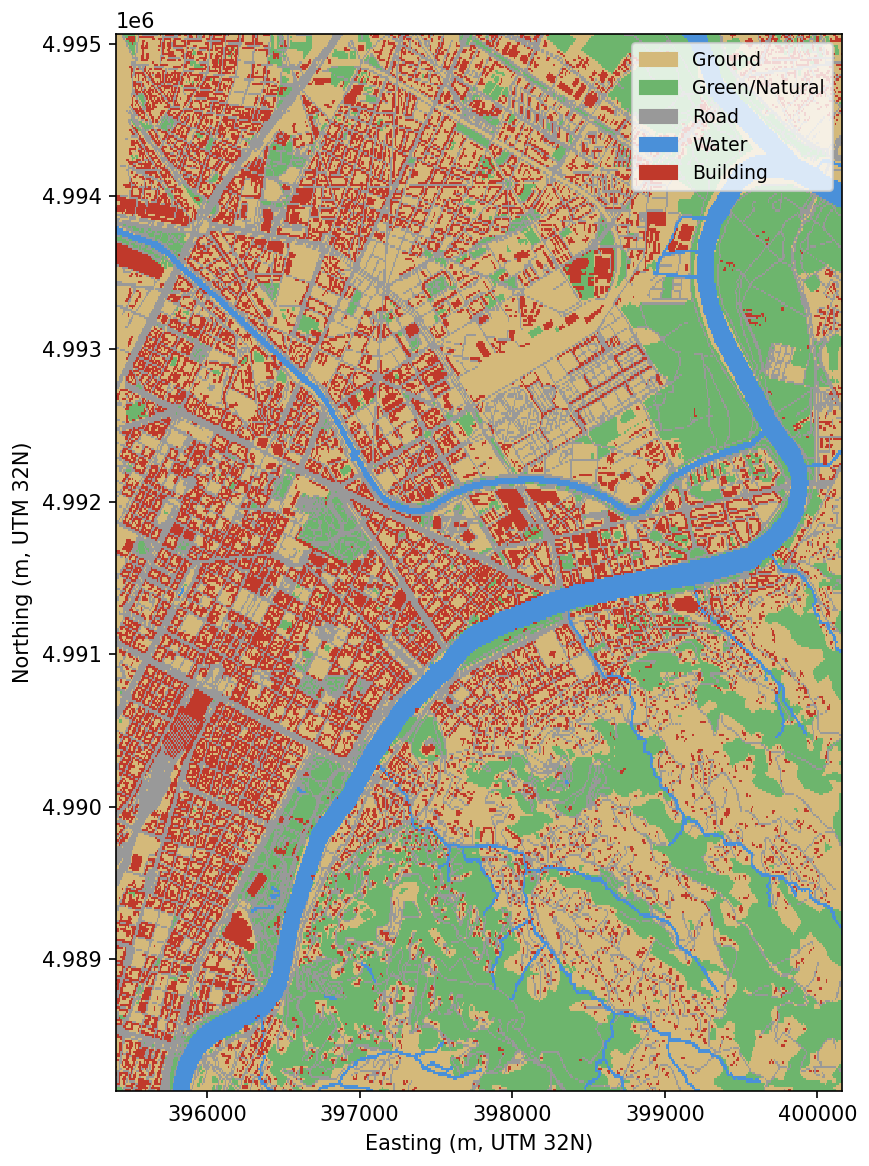
\includegraphics[height=0.42\textheight, keepaspectratio]{figures/chap4/step0/TERRAIN_MAP_cropped.png}
    \caption[Classified terrain grid of the area of interest]{Classified terrain grid of the area of interest in UTM coordinates (Zone 32N), with $500 \times 500$ cells of approximately 9.5\,m $\times$ 13.8\,m, each assigned to one of the five categories \texttt{WATER}, \texttt{BUILDINGS}, \texttt{ROADS}, \texttt{GREEN/NATURAL}, and \texttt{GROUND}.}
    \label{fig:terrain-map}
\end{figure}

\subsubsection{Mission trajectory definition}
% route endpoints (hospitals), B-spline trajectory, cruise altitude and speed
This step aims to define the trajectory above the map produced earlier. The waypoints of the trajectory (a collection of manually-selected points retracing the routes proposed in Section \ref{sec:reference-mission}, defined in degrees of latitude and longitude and stored in an external Excel file) are loaded and checked against the bounding box of the map, ensuring that any waypoint falling outside it is discarded. The waypoints are then converted to UTM metres (zone 32N, EPSG:32632), with the same transformation used for the map, and interpolated with a cubic B-spline using the \texttt{splprep} function of SciPy. No smoothing is applied ($s = 0$), so the curve passes exactly through every waypoint. The spline is parametric, i.e. $x$ and $y$ are both expressed as functions of a parameter $t \in [0, 1]$, and the curve is made of cubic polynomials joined at the waypoints with continuous first and second derivatives. If fewer than four valid waypoints are available, the code falls back to straight line segments ($k = 1$).

Then, points every 10\,m along the curve are extracted through an arclength parametrisation. The spline is evaluated at 100\,000 equally spaced values of $t$, and the cumulative arclength is computed by summing the lengths of the straight segments between consecutive points. The values of $t$ that correspond to every 10\,m of distance are found by linear interpolation on this cumulative arclength and saved with the new label $t^*$, and the spline is evaluated at these values to give the points where the evaluation is conducted later. The same goes for the heading angle, computed at every sample point from the local direction of the trajectory and measured counterclockwise from East. The sample points guarantee a high level of accuracy because, for a total length of about 11\,km, consecutive spline points $t$ are about 0.11\,m apart, so there are about 90 of them for every sample point $t^*$. The trajectories following Route A and Route B are shown in Fig.\ref{fig:trajectories}.

\begin{figure}[htbp]
    \centering
    \begin{subfigure}[b]{0.48\textwidth}
        \centering
        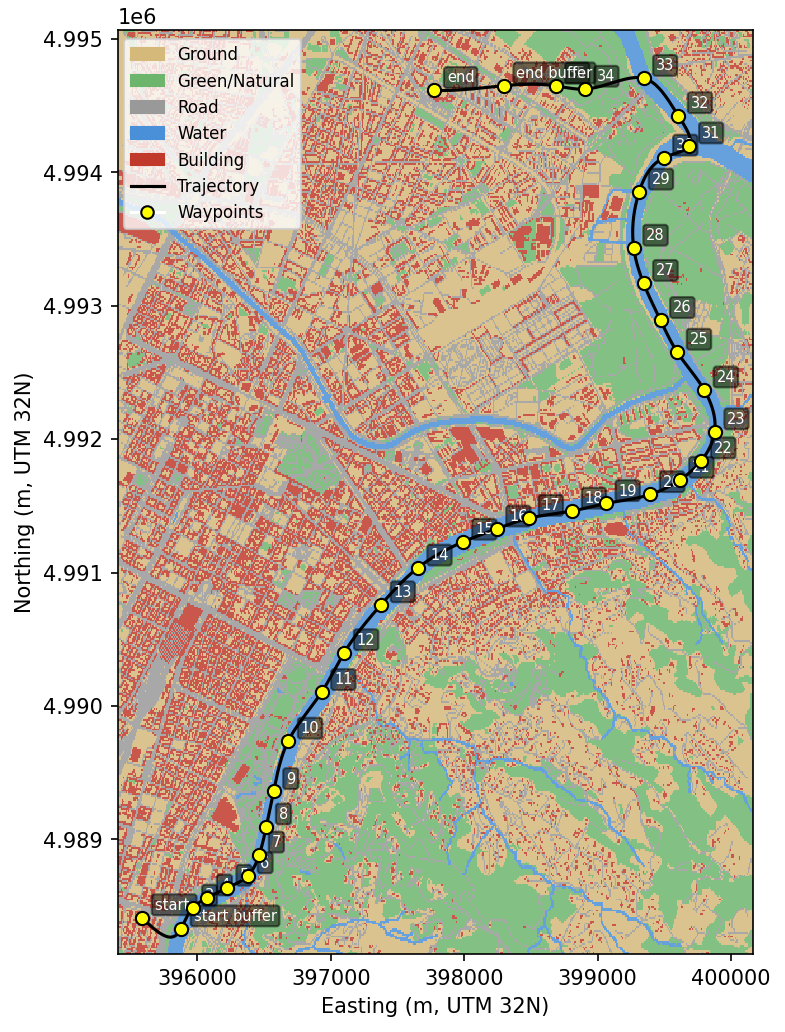
\includegraphics[width=\textwidth]{figures/chap4/step0/TERRAIN_MAP_with_trajectory_PO-e-STURA_notitle.png}
        \caption{Route A (above-the-river trajectory along the Po and the Stura).}
        \label{fig:trajectory-routeA}
    \end{subfigure}
    \hfill
    \begin{subfigure}[b]{0.48\textwidth}
        \centering
        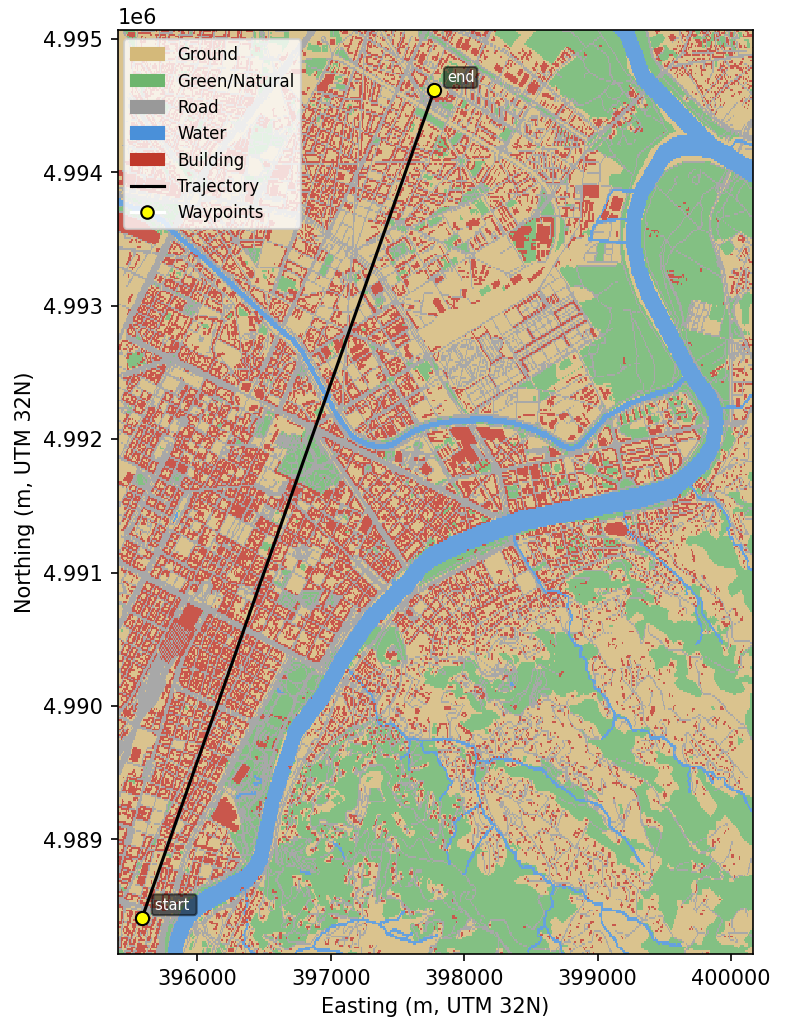
\includegraphics[width=\textwidth]{figures/chap4/step0/TERRAIN_MAP_with_trajectory_STRAIGHT-LINE_notitle.png}
        \caption{Route B (straight-line trajectory over the city).}
        \label{fig:trajectory-routeB}
    \end{subfigure}
    \caption[Mission trajectories over the classified terrain grid]{Mission trajectories over the classified terrain grid in UTM coordinates (Zone 32N), from the Molinette Hospital (start) to the San Giovanni Bosco Hospital (end): (a) Route A, interpolated with a cubic B-spline through the numbered waypoints; (b) Route B, a straight segment between the two endpoints.}
    \label{fig:trajectories}
\end{figure}

\subsubsection{Failure and fall model}
% failure scenario (where along the route, initial state at failure)
% equations of motion: gravity + drag (Cd, area, mass), integration scheme
% wind: included or not

As described in Section \ref{sec:reference-mission}, the reference mission scenario assumes that, in case of UAV failure with uncontrolled descent, the payload is detached from the drone and falls with no propulsion or control mechanism. Therefore, the equations of motion that determine its trajectory must include only the gravitational contribution and the aerodynamic contribution, the latter through a drag term. Given the air density $\rho$, the frontal area of the payload $S$ and the drag coefficient $C_d$, the drag force is
\begin{equation}
  F_d = c\,V^2, \qquad c = \frac{1}{2}\,\rho\,S\,C_d ,
  \label{eq:drag}
\end{equation}
where $V$ is the instantaneous speed of the payload.

For every combination of parameters, the drag constant $c$ is calculated first, and then the terminal velocity
\begin{equation}
  \Gamma = \sqrt{\frac{M\,g}{c}} ,
  \label{eq:terminal_velocity}
\end{equation}
i.e. the maximum vertical speed the payload can reach, at which drag balances gravity. For the payload considered here ($M = 1.0$\,kg, $\rho=1.225$kg/m$^3$, $S = 0.04$\,m$^2$, $C_d \approx 1.0$), $\Gamma \approx 20.0$~m/s.


The descent is then divided into three phases. Firstly, there is an "upward motion phase", present only if the payload has an upward vertical velocity at separation. Secondly, there is a primary descent phase in which the vertical velocity is lower than the horizontal velocity, which ends when the two become equal. Finally, there is the final descent phase from this crossing to the ground, in which the vertical velocity catches up and approaches $\Gamma$ while the horizontal velocity keeps decreasing. Each phase has its own approximate closed-form expressions for position and velocity based on the model presented by Angelini (2023) \cite{Angelini2023}. The horizontal range is the sum of the distances covered in the three phases, and the effects of the wind and drag are taken into account throughout the calculation for both the vertical and the horizontal velocities.

The conditions at the moment of drone-payload separation cannot be predicted exactly for each single flight. For this reason, some parameters are modelled through a Gaussian distribution, each described by a mean $\mu$ and a standard deviation $\sigma$, and sampled randomly at each simulation, as listed in Table~\ref{tab:uncertain_params}.

\begin{table}[htbp]
  \centering
  \caption{Uncertain parameters of the drop model, each sampled from a Gaussian distribution.}
  \label{tab:uncertain_params}
  \begin{thesistable}{
    colspec = {X[1.5,l] Q[l] Q[c] Q[c] X[1.6,l]},
  }
    Parameter & Unit & $\mu$ & $\sigma$ & Remarks \\
    Altitude at separation $h$ & m & 75 & 5 & Small variations in flight altitude \\
    Drag coefficient $C_d$ & - & 1.0 & 0.2 & Payload tumbling or rotation\\
    Horizontal velocity at separation $V_{x,i}$ & m/s & 17 & 6 & Inherited from the drone cruise speed \\
    Vertical velocity at separation $V_{y,i}$ & m/s & 0 & 0.5 & Zero mean assumes level flight at failure \\
    Wind speed $V_w$ & m/s & 15 & 0 & Assuming a constant, high wind speed for conservative calculations\\
    Wind direction $\psi_w$ & deg & 0 & 360 & A large $\sigma$ produces a wide lateral spread \\
  \end{thesistable}
\end{table}

\subsubsection{Monte Carlo impact loop}
% sampled variables + their distributions
% number of samples, convergence criterion
For each point $t^*$ of the trajectory calculated earlier, i.e. for every point corresponding to a distance of 10\,m along the curve, a Monte Carlo simulation is run with 5000 combinations of the stochastic parameters, selected randomly from the Gaussian distributions of Table \ref{tab:uncertain_params}. Having established these parameter combinations coupled with information on UAV heading direction at single $t^*$ points, the function \texttt{impact\_point\_ballistic\_descent} is called to calculate where the trajectory and the landing location of the payload. The function computes the horizontal range and the impact time of all 5000 scenarios at once and rotates the resulting cloud of impact points by the heading, so that it is oriented along the flight direction. Each impact point is then shifted by the wind drift $V_w\,t_{im}$ in the wind direction, assuming that the wind carries the payload at its own speed for the whole duration of the fall, and the cloud is finally translated to the UTM coordinates of the trajectory point.

The impact points are then counted on a grid of cells [$2000 \times 2000$], finer than the one used for the terrain map to guarantee higher accuracy in computing the impact distribution. As each trajectory point this gives a local distribution, the local distributions of all the $t^*$ points are summed up with equal weight and normalised over the total number of impact events, i.e. 5000 times the number of  $t^*$ points on the trajectory. At the end of the Monte Carlo simulation, the heatmap in Figure~\ref{fig:heatmap} is obtained, which gives, for each cell, the probability that the payload falls in that cell in case of a failure along the trajectory.

\begin{figure}[htbp]
    \centering
    \begin{subfigure}[b]{0.48\textwidth}
        \centering
        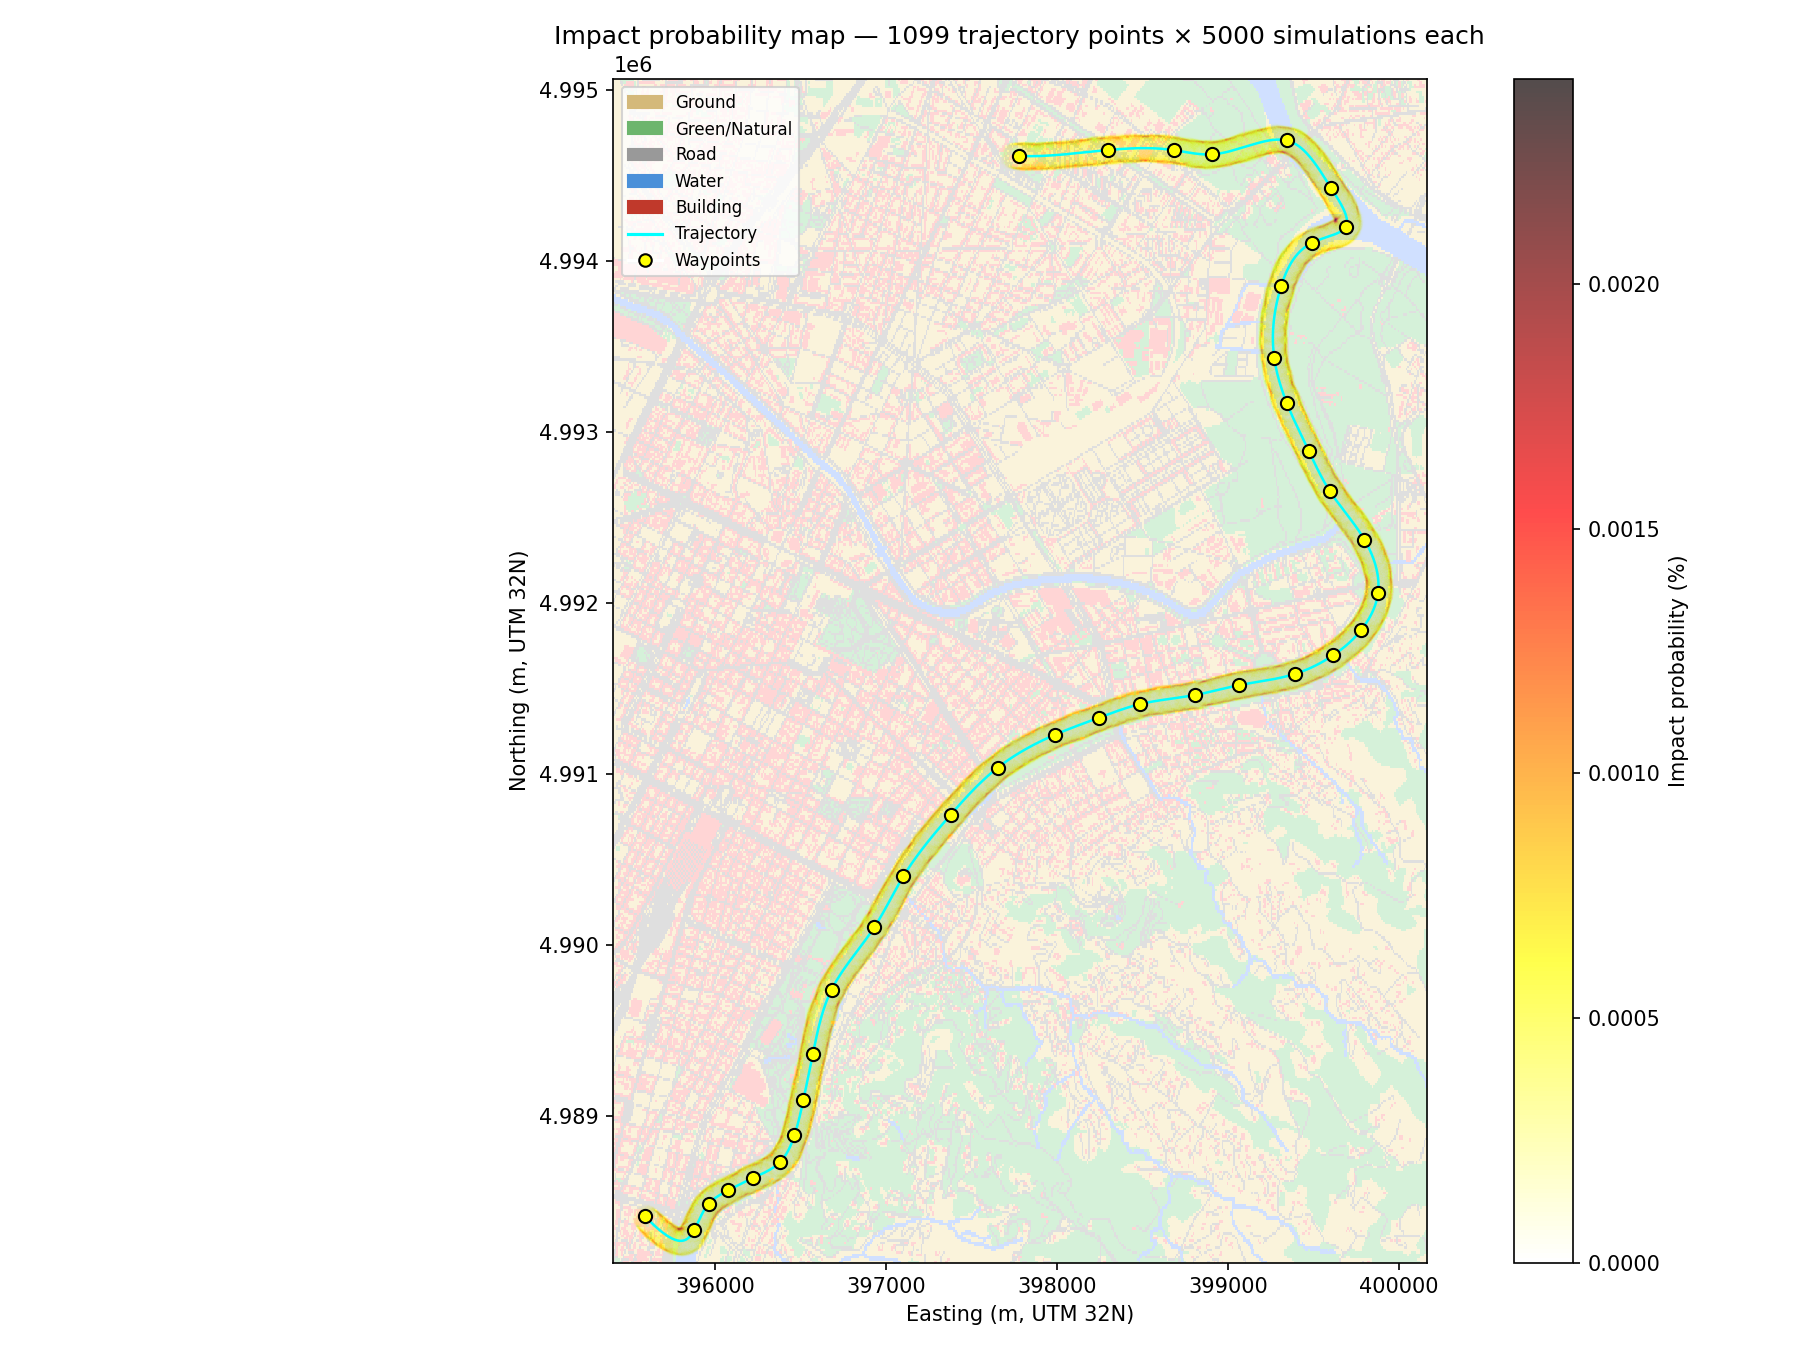
\includegraphics[width=\textwidth, trim=235 0 38 25, clip]{figures/chap4/step0/PO-e-STURA_impact_heatmap.png}
        \caption{Route A (above-the-river trajectory along the Po and the Stura).}
        \label{fig:heatmap-routeA}
    \end{subfigure}
    \hfill
    \begin{subfigure}[b]{0.48\textwidth}
        \centering
        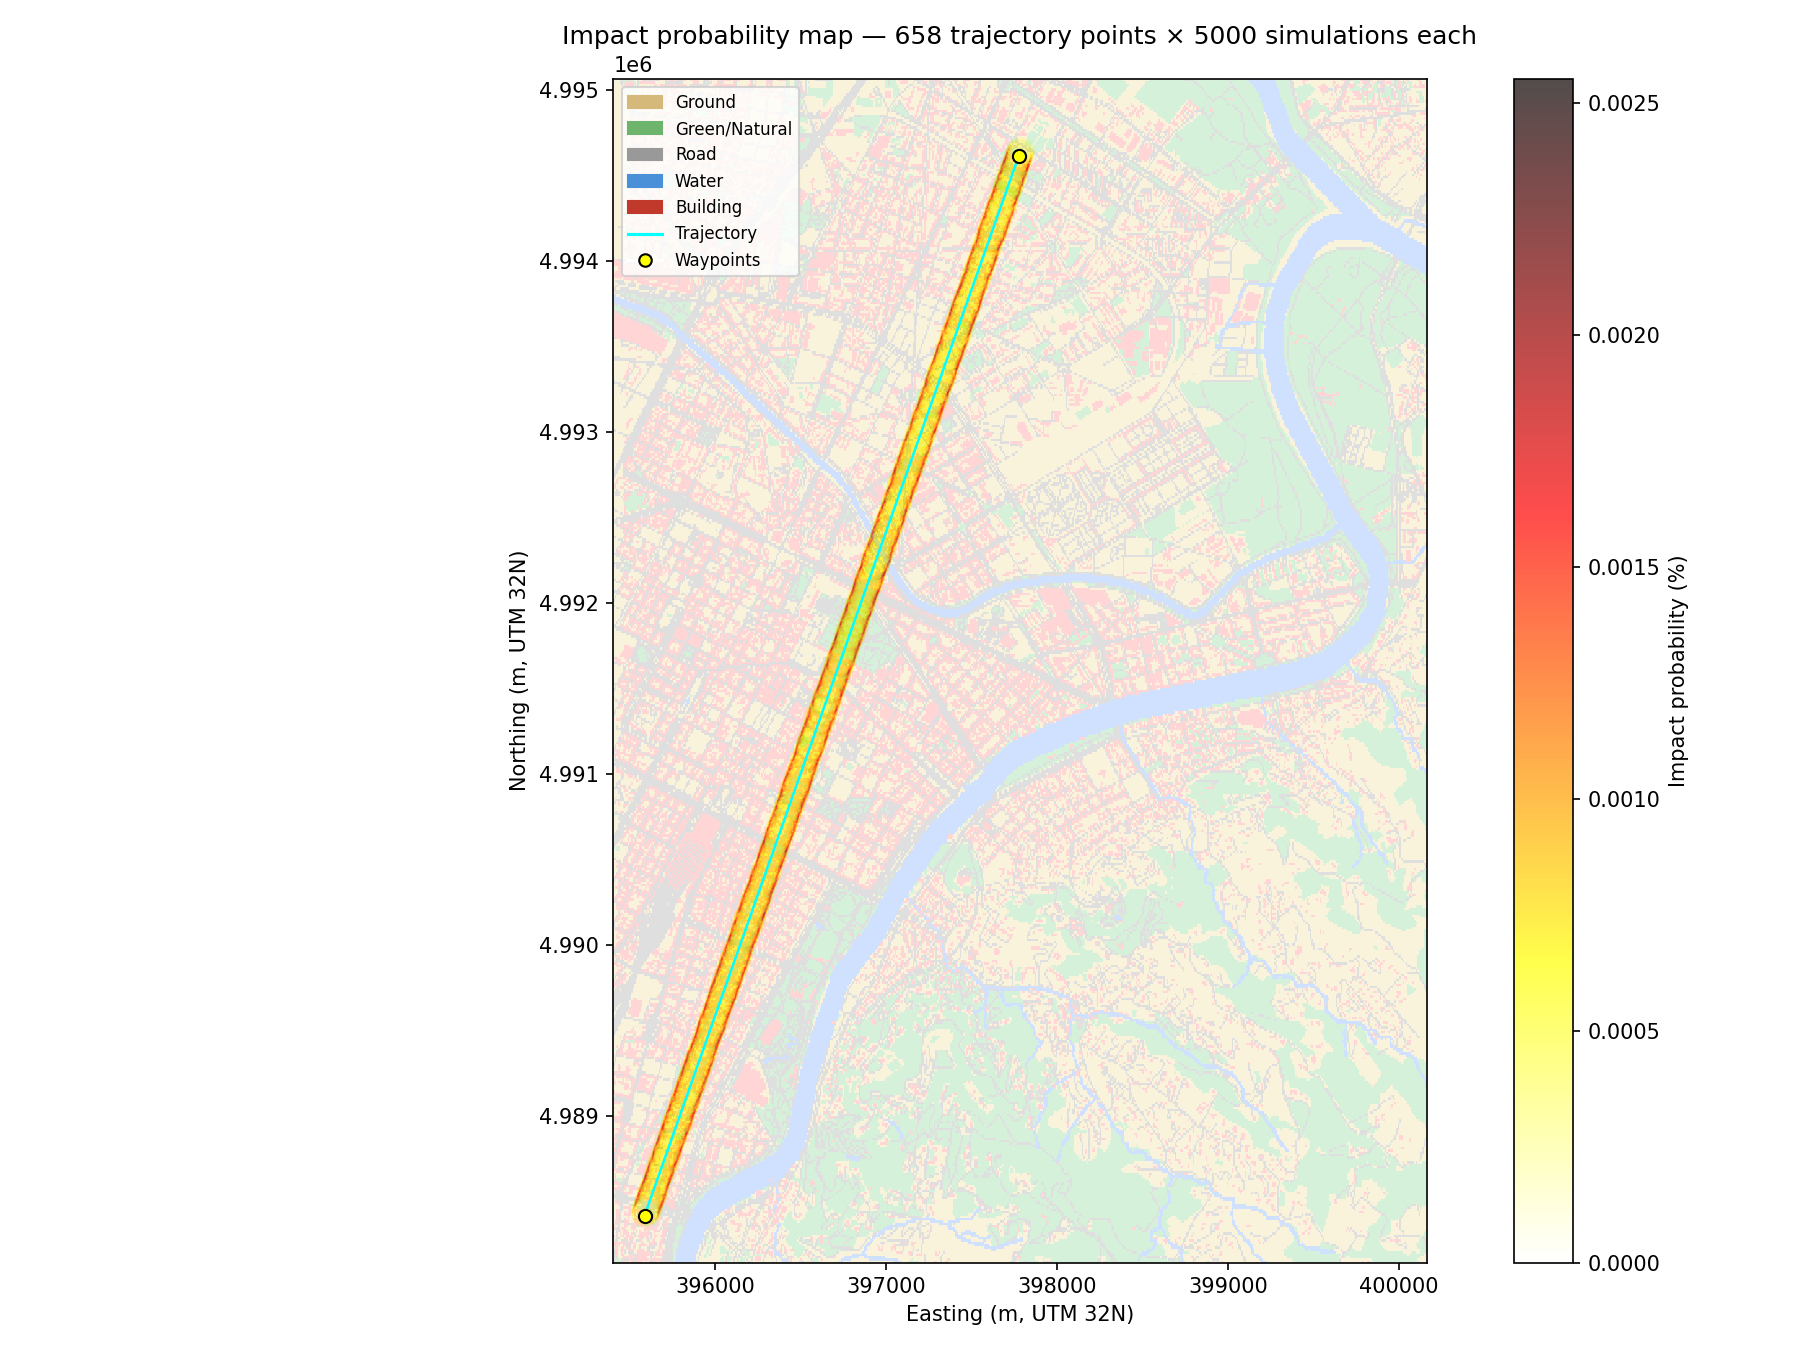
\includegraphics[width=\textwidth, trim=235 0 38 25, clip]{figures/chap4/step0/STRAIGHT-LINE_impact_heatmap.png}
        \caption{Route B (straight-line trajectory over the city).}
        \label{fig:heatmap-routeB}
    \end{subfigure}
    \caption[Impact probability maps along the mission trajectories]{Impact probability maps over the classified terrain grid in UTM coordinates (Zone 32N), obtained with 5000 Monte Carlo simulations per trajectory point and expressed as the probability (\%) that the payload falls in each cell in case of a failure along the route: (a) Route A, 1099 trajectory points; (b) Route B, 658 trajectory points.}
    \label{fig:heatmap}
\end{figure}



\subsection{Results}
\subsubsection{Convergence of the Monte Carlo}  % running mean/percentiles vs N
taking statistically significant number of samples, and also considering a statistically significant number of points above or below high or low percentiles (e.g. if there's only 1 data point above the 99th percentile, then you don't consider it)
\subsubsection{Impact location distribution}   % density map over Turin
\subsubsection{Impact conditions}             % velocity (and angle) histograms + percentiles
\subsubsection{Impact surface statistics}     % ground/roof/facade fractions
\subsubsection{Design inputs for the following steps} % the chosen velocity percentile -> airbag
\subsubsection{Limitations}                   % map resolution, no wind, drag model, etc.



\subsubsection{Step 0 deliverable: impact velocities and free-fall time}






